\documentclass{standalone}
\usepackage{tikz}
\usetikzlibrary{patterns, positioning}
\usepackage[sfdefault]{ClearSans} %% option 'sfdefault' activates Clear Sans as the default text font
\usepackage[T1]{fontenc}

\begin{document}
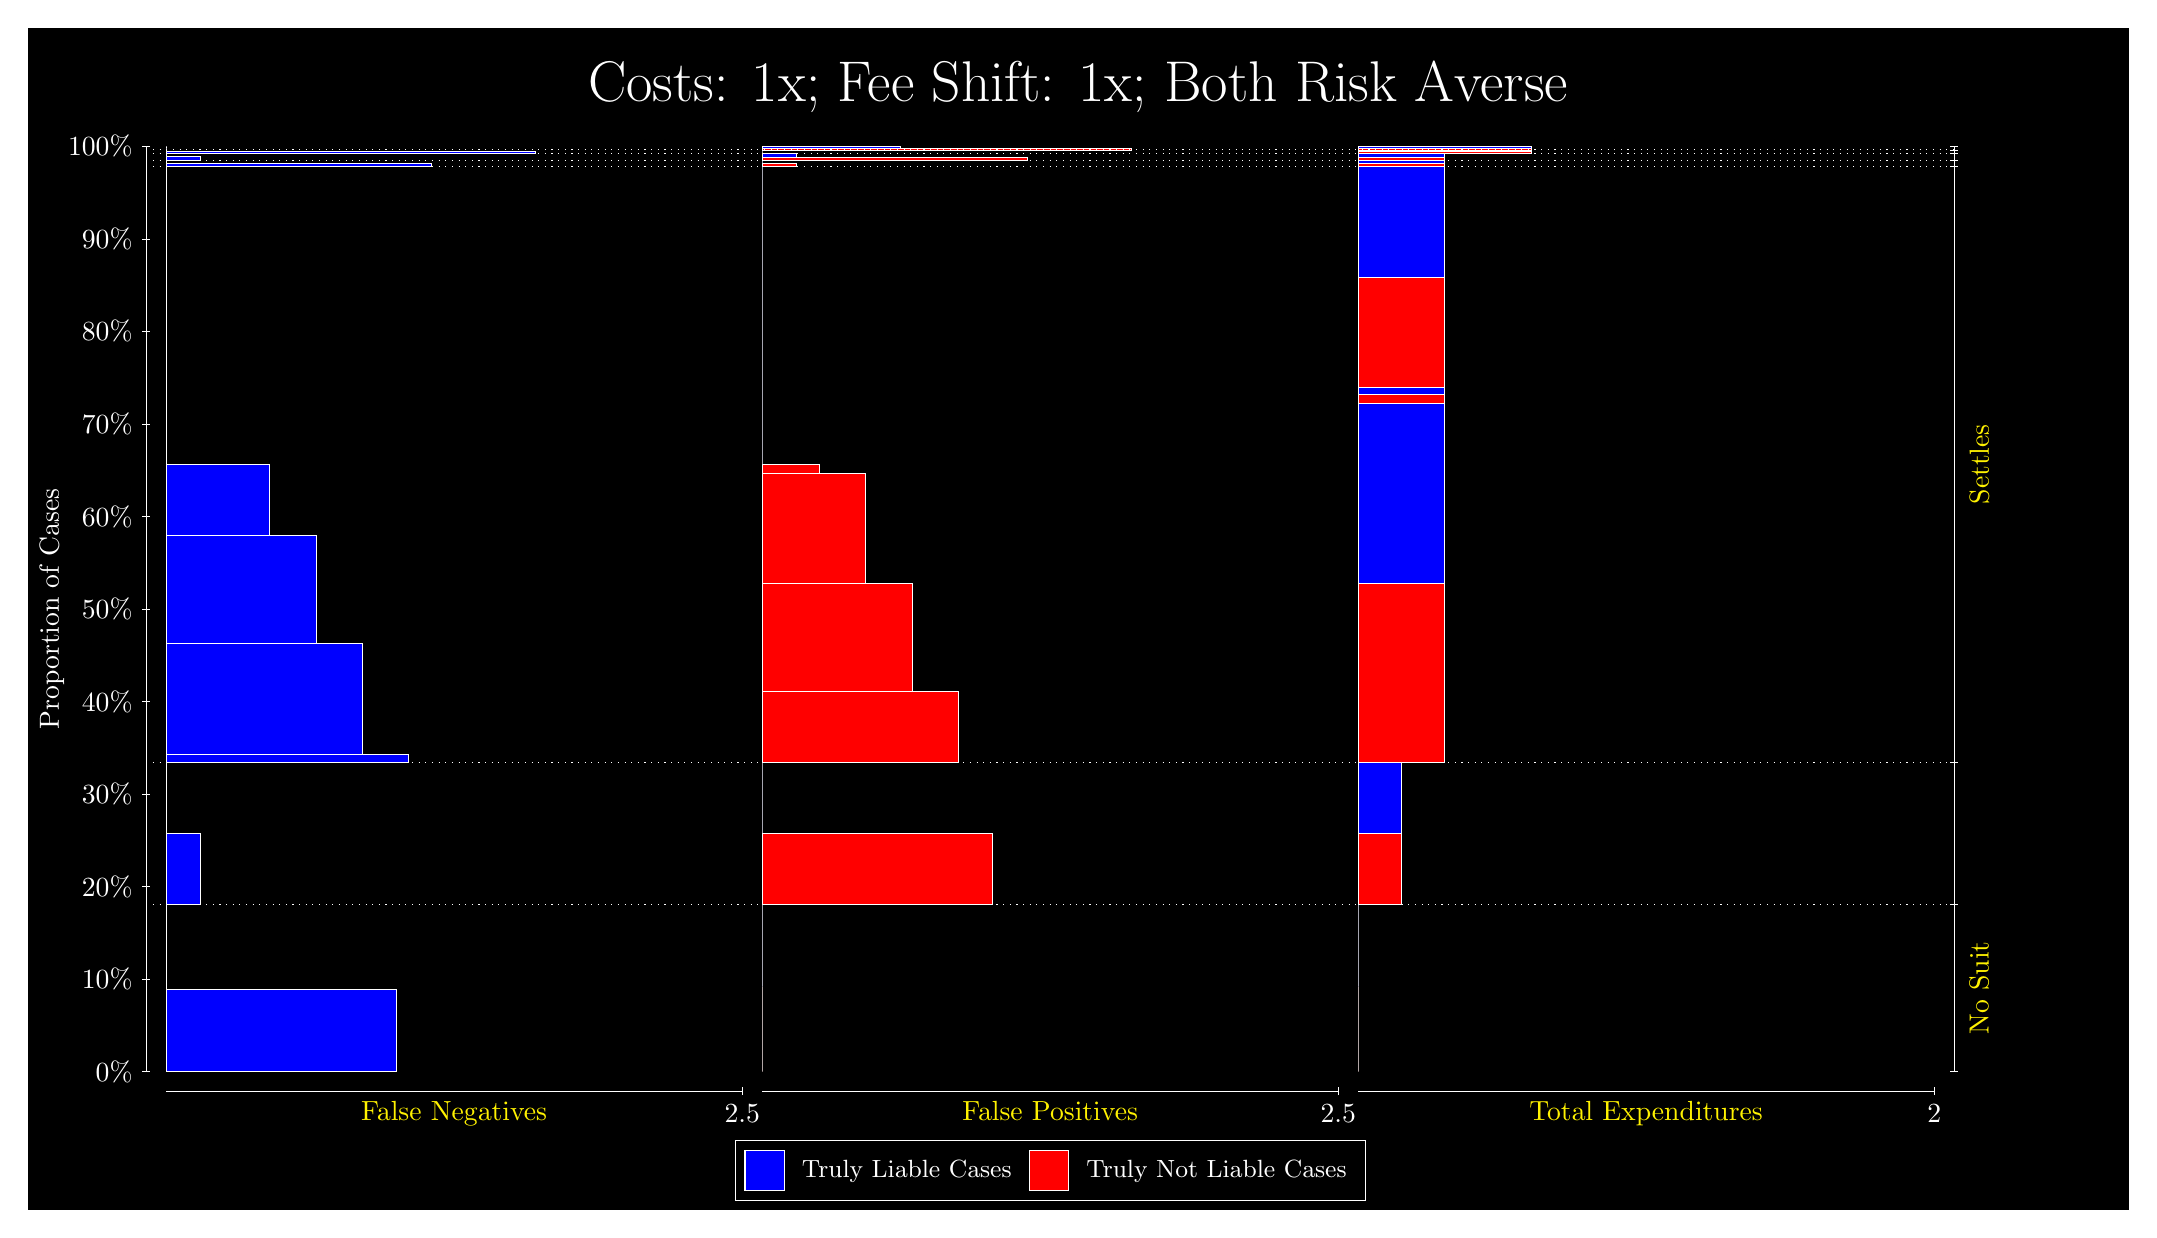
\begin{tikzpicture}
\draw[fill=black] (0,0) rectangle (26.667,15);
\draw[text=white] (0,13.5) rectangle (26.667,15) node[midway] {\huge Costs: 1x; Fee Shift: 1x; Both Risk Averse};
\draw[white, very thin] (1.5,1.75) -- (1.5,13.5);
\node[rotate=90, text=white, anchor=center] at (0.3, 7.625) {Proportion of Cases};
\draw[white, very thin] (1.45,1.75) -- (1.55,1.75);
\node[text=white, anchor=east] at (1.45, 1.75) {0\%};
\draw[white, very thin] (1.45,2.925) -- (1.55,2.925);
\node[text=white, anchor=east] at (1.45, 2.925) {10\%};
\draw[white, very thin] (1.45,4.1) -- (1.55,4.1);
\node[text=white, anchor=east] at (1.45, 4.1) {20\%};
\draw[white, very thin] (1.45,5.275) -- (1.55,5.275);
\node[text=white, anchor=east] at (1.45, 5.275) {30\%};
\draw[white, very thin] (1.45,6.45) -- (1.55,6.45);
\node[text=white, anchor=east] at (1.45, 6.45) {40\%};
\draw[white, very thin] (1.45,7.625) -- (1.55,7.625);
\node[text=white, anchor=east] at (1.45, 7.625) {50\%};
\draw[white, very thin] (1.45,8.8) -- (1.55,8.8);
\node[text=white, anchor=east] at (1.45, 8.8) {60\%};
\draw[white, very thin] (1.45,9.975) -- (1.55,9.975);
\node[text=white, anchor=east] at (1.45, 9.975) {70\%};
\draw[white, very thin] (1.45,11.15) -- (1.55,11.15);
\node[text=white, anchor=east] at (1.45, 11.15) {80\%};
\draw[white, very thin] (1.45,12.325) -- (1.55,12.325);
\node[text=white, anchor=east] at (1.45, 12.325) {90\%};
\draw[white, very thin] (1.45,13.5) -- (1.55,13.5);
\node[text=white, anchor=east] at (1.45, 13.5) {100\%};

\draw[white, very thin] (24.457,1.75) -- (24.457,13.5);
\draw[white, very thin] (24.407,1.75) -- (24.507,1.75);
\node[anchor=west] at (24.407, 1.75) {};
\draw[white, very thin] (24.407,3.8727) -- (24.507,3.8727);
\node[anchor=west] at (24.407, 3.8727) {};
\draw[white, very thin] (24.407,5.6803) -- (24.507,5.6803);
\node[anchor=west] at (24.407, 5.6803) {};
\draw[white, very thin] (24.407,13.244) -- (24.507,13.244);
\node[anchor=west] at (24.407, 13.244) {};
\draw[white, very thin] (24.407,13.319) -- (24.507,13.319);
\node[anchor=west] at (24.407, 13.319) {};
\draw[white, very thin] (24.407,13.41) -- (24.507,13.41);
\node[anchor=west] at (24.407, 13.41) {};
\draw[white, very thin] (24.407,13.454) -- (24.507,13.454);
\node[anchor=west] at (24.407, 13.454) {};
\draw[white, very thin] (24.407,13.5) -- (24.507,13.5);
\node[anchor=west] at (24.407, 13.5) {};

\draw[white, very thin, fill=blue] (1.75,1.75) rectangle (4.6775,2.7951);
\draw[white, very thin, fill=red] (1.75,2.7951) rectangle (1.75,3.8727);
\draw[white, very thin, fill=blue] (1.75,3.8727) rectangle (2.1891,4.7765);
\draw[white, very thin, fill=red] (1.75,4.7765) rectangle (1.75,5.6803);
\draw[white, very thin, fill=blue] (1.75,5.6803) rectangle (4.8239,5.7813);
\draw[white, very thin, fill=blue] (1.75,5.7813) rectangle (4.2384,7.1857);
\draw[white, very thin, fill=blue] (1.75,7.1857) rectangle (3.6529,8.5624);
\draw[white, very thin, fill=blue] (1.75,8.5624) rectangle (3.0674,9.4662);
\draw[white, very thin, fill=red] (1.75,9.4662) rectangle (1.75,13.244);
\draw[white, very thin, fill=blue] (1.75,13.244) rectangle (5.1167,13.282);
\draw[white, very thin, fill=red] (1.75,13.282) rectangle (1.75,13.319);
\draw[white, very thin, fill=blue] (1.75,13.319) rectangle (2.1891,13.373);
\draw[white, very thin, fill=red] (1.75,13.373) rectangle (1.75,13.41);
\draw[white, very thin, fill=blue] (1.75,13.41) rectangle (6.4341,13.432);
\draw[white, very thin, fill=red] (1.75,13.432) rectangle (1.75,13.454);
\draw[white, very thin, fill=red] (1.75,13.454) rectangle (1.75,13.474);
\draw[white, very thin, fill=blue] (1.75,13.474) rectangle (1.75,13.5);
\draw[white, very thin, fill=red] (9.3189,1.75) rectangle (9.3189,2.8275);
\draw[white, very thin, fill=blue] (9.3189,2.8275) rectangle (9.3189,3.8727);
\draw[white, very thin, fill=red] (9.3189,3.8727) rectangle (12.246,4.7765);
\draw[white, very thin, fill=blue] (9.3189,4.7765) rectangle (9.3189,5.6803);
\draw[white, very thin, fill=red] (9.3189,5.6803) rectangle (11.807,6.5842);
\draw[white, very thin, fill=red] (9.3189,6.5842) rectangle (11.222,7.9547);
\draw[white, very thin, fill=red] (9.3189,7.9547) rectangle (10.636,9.3491);
\draw[white, very thin, fill=red] (9.3189,9.3491) rectangle (10.051,9.4585);
\draw[white, very thin, fill=blue] (9.3189,9.4585) rectangle (9.3189,13.244);
\draw[white, very thin, fill=red] (9.3189,13.244) rectangle (9.758,13.281);
\draw[white, very thin, fill=blue] (9.3189,13.281) rectangle (9.3189,13.319);
\draw[white, very thin, fill=red] (9.3189,13.319) rectangle (12.686,13.355);
\draw[white, very thin, fill=blue] (9.3189,13.355) rectangle (9.758,13.41);
\draw[white, very thin, fill=red] (9.3189,13.41) rectangle (9.3189,13.432);
\draw[white, very thin, fill=blue] (9.3189,13.432) rectangle (9.3189,13.454);
\draw[white, very thin, fill=red] (9.3189,13.454) rectangle (14.003,13.474);
\draw[white, very thin, fill=blue] (9.3189,13.474) rectangle (11.075,13.5);
\draw[white, very thin, fill=red] (16.888,1.75) rectangle (16.888,2.8275);
\draw[white, very thin, fill=blue] (16.888,2.8275) rectangle (16.888,3.8727);
\draw[white, very thin, fill=red] (16.888,3.8727) rectangle (17.437,4.7765);
\draw[white, very thin, fill=blue] (16.888,4.7765) rectangle (17.437,5.6803);
\draw[white, very thin, fill=red] (16.888,5.6803) rectangle (17.986,7.9547);
\draw[white, very thin, fill=blue] (16.888,7.9547) rectangle (17.986,10.235);
\draw[white, very thin, fill=red] (16.888,10.235) rectangle (17.986,10.345);
\draw[white, very thin, fill=blue] (16.888,10.345) rectangle (17.986,10.446);
\draw[white, very thin, fill=red] (16.888,10.446) rectangle (17.986,11.84);
\draw[white, very thin, fill=blue] (16.888,11.84) rectangle (17.986,13.244);
\draw[white, very thin, fill=red] (16.888,13.244) rectangle (17.986,13.281);
\draw[white, very thin, fill=blue] (16.888,13.281) rectangle (17.986,13.319);
\draw[white, very thin, fill=red] (16.888,13.319) rectangle (17.986,13.355);
\draw[white, very thin, fill=blue] (16.888,13.355) rectangle (17.986,13.41);
\draw[white, very thin, fill=red] (16.888,13.41) rectangle (19.083,13.432);
\draw[white, very thin, fill=blue] (16.888,13.432) rectangle (19.083,13.454);
\draw[white, very thin, fill=red] (16.888,13.454) rectangle (19.083,13.474);
\draw[white, very thin, fill=blue] (16.888,13.474) rectangle (19.083,13.5);
\draw[white, dotted] (1.5,3.8727) -- (24.457,3.8727);
\draw[white, dotted] (1.5,5.6803) -- (24.457,5.6803);
\draw[white, dotted] (1.5,13.244) -- (24.457,13.244);
\draw[white, dotted] (1.5,13.319) -- (24.457,13.319);
\draw[white, dotted] (1.5,13.41) -- (24.457,13.41);
\draw[white, dotted] (1.5,13.454) -- (24.457,13.454);
\draw[white, very thin] (1.75,1.5) -- (9.0689,1.5);
\node[text=yellow, anchor=north] at (5.4094, 1.5) {False Negatives};
\draw[white, very thin] (9.0689,1.45) -- (9.0689,1.55);
\node[text=white, anchor=north] at (9.0689, 1.45) {2.5};

\draw[white, very thin] (9.3189,1.5) -- (16.638,1.5);
\node[text=yellow, anchor=north] at (12.978, 1.5) {False Positives};
\draw[white, very thin] (16.638,1.45) -- (16.638,1.55);
\node[text=white, anchor=north] at (16.638, 1.45) {2.5};

\draw[white, very thin] (16.888,1.5) -- (24.207,1.5);
\node[text=yellow, anchor=north] at (20.547, 1.5) {Total Expenditures};
\draw[white, very thin] (24.207,1.45) -- (24.207,1.55);
\node[text=white, anchor=north] at (24.207, 1.45) {2};

\node[text=yellow, centered, rotate=90] at (24.777, 2.8113) {No Suit};

\node[text=yellow, centered, rotate=90] at (24.777, 9.4624) {Settles};





\draw (12.978300999999998,1.5) node[draw=none] (baseCoordinate) {};
\begin{scope}[align=center]
        \matrix[scale=0.5, draw=white, below=0.5cm of baseCoordinate, nodes={draw}, column sep=0.1cm]{
            \node[rectangle, draw, minimum width=0.5cm, minimum height=0.5cm, fill=blue] {}; &
            \node[draw=none, font=\small, text=white] (B) {Truly Liable Cases}; &
            \node[rectangle, draw, minimum width=0.5cm, minimum height=0.5cm, fill=red] {}; &
            \node[draw=none, font=\small, text=white] (B) {Truly Not Liable Cases}; \\
            };
\end{scope}

\end{tikzpicture}
\end{document}